\chapter{Methodology}


This section outlines the system architecture, tools, datasets, and evaluation protocols employed to design and assess the proposed framework that substitutes traditional Regular Expressions (RegEx) with a hybrid solution leveraging Retrieval-Augmented Generation (RAG) and Agentic AI. The methodology is structured around four core components:


\section{Core System Architecture}

The core system combines Retrieval-Augmented Generation (RAG)~\cite{lewis2020rag,zhang2024survey} with a modular agentic planner~\cite{ft2024agents} to transform natural language instructions into actionable information extraction routines. The RAG subsystem handles knowledge grounding through a dual-phase retrieval and generation process, leveraging mechanisms explored in frameworks like Ext2Gen~\cite{chen2024ext2gen} and HybridRAG~\cite{kabir2024hybridrag} to improve alignment and accuracy. Meanwhile, the agentic controller selects and sequences tools based on the semantic intent of the input, embodying goal-driven behavior, memory usage, and reflective reasoning capabilities as described in recent advances in Agentic AI~\cite{ft2024agents} (see Figure~\ref{fig:agentic_rag_architecture}). 

\vspace{0.5cm}

\section{Core Components of RAG}

The architecture of Retrieval-Augmented Generation (RAG) systems integrates three primary components (see Figure~\ref{fig:rag_architecture}): 
\begin{itemize}
    \item \textbf{Retrieval:} Responsible for querying external data sources such as knowledge bases, APIs, or vector databases. Advanced retrievers leverage dense vector search and transformer-based models to improve retrieval precision and semantic relevance \cite{lewis2020retrieval}.
    \item \textbf{Augmentation:} Processes retrieved data, extracting and summarizing the most relevant information to align with the query context.
    \item \textbf{Generation:} Combines retrieved information with the LLM’s pre-trained knowledge to generate coherent, contextually appropriate responses \cite{lewis2020retrieval}.
\end{itemize}

\begin{figure}[h!]
    \centering
    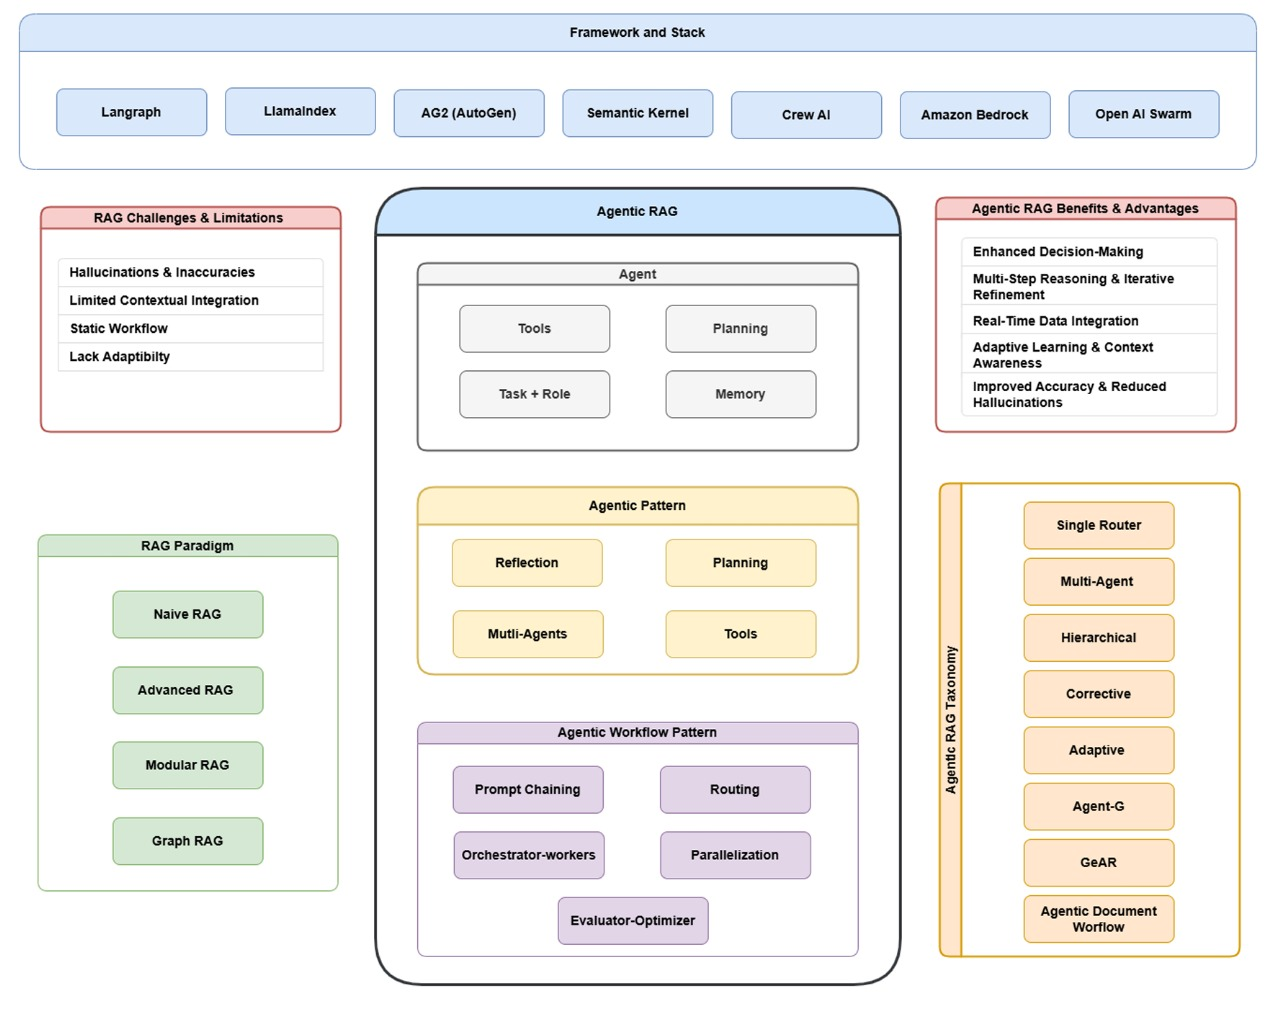
\includegraphics[width=0.95\textwidth]{images/fig_1.jpg}
    \caption{
        \textbf{Agentic RAG Framework and Taxonomy.}
        This figure presents the integration of Retrieval-Augmented Generation (RAG) with agentic planning. The architecture highlights the interaction between the retrieval, augmentation, and generation modules, coordinated by an agentic controller that enables dynamic tool selection, memory utilization, and reflective reasoning for robust information extraction.
    }
    \label{fig:agentic_rag_architecture}
\end{figure}

\begin{figure}[h!]
    \centering
    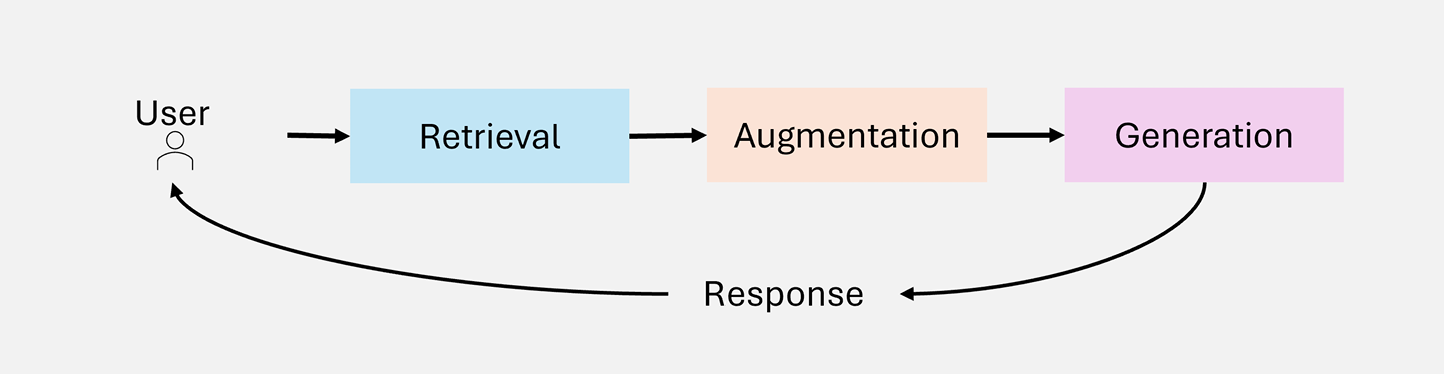
\includegraphics[width=0.9\linewidth]{images/fig_2.png}
    \caption{
        \textbf{Architecture of the Retrieval-Augmented Generation (RAG) System.}
        The diagram illustrates the three core components: (1) \emph{Retrieval}, which queries external knowledge sources using dense vector search and transformer-based models; (2) \emph{Augmentation}, which processes and filters retrieved data to maximize contextual relevance; and (3) \emph{Generation}, where the LLM synthesizes responses by integrating retrieved knowledge with its internal representations. This modular pipeline enables dynamic, context-aware information extraction and response generation.
    }
    \label{fig:rag_architecture}
\end{figure}


\section{Evolution of RAG Paradigms}

The field of Retrieval-Augmented Generation (RAG) has evolved significantly to address the increasing complexity of real-world applications, where contextual accuracy, scalability, and multi-step reasoning are critical. What began as simple keyword-based retrieval has transitioned into sophisticated, modular, and adaptive systems capable of integrating diverse data sources and autonomous decision-making processes~\cite{lewis2020retrieval,kabir2024hybridrag,chen2024ext2gen}. This evolution underscores the growing need for RAG systems to handle complex queries efficiently and effectively.

This section examines the progression of RAG paradigms, presenting key stages of development---Naïve RAG, Advanced RAG, Modular RAG, Graph RAG, and Agentic RAG---alongside their defining characteristics, strengths, and limitations. By understanding the evolution of these paradigms, readers can appreciate the advancements made in retrieval and generative capabilities and their application in various domains.


\subsection{Naïve RAG}
Naïve RAG \cite{lewis2020retrieval} represents the foundational implementation of retrieval-augmented generation. Figure~\ref{fig:naive_rag_architecture} illustrates the simple retrieve-read workflow of Naïve RAG, which focuses on keyword-based retrieval and the use of static datasets. These systems rely on conventional retrieval techniques such as TF-IDF and BM25 to fetch relevant documents. The retrieved texts are subsequently used to augment the language model’s generative capabilities, enabling improved contextual coherence without the need for real-time adaptability.

\begin{figure}[h!]
    \centering
    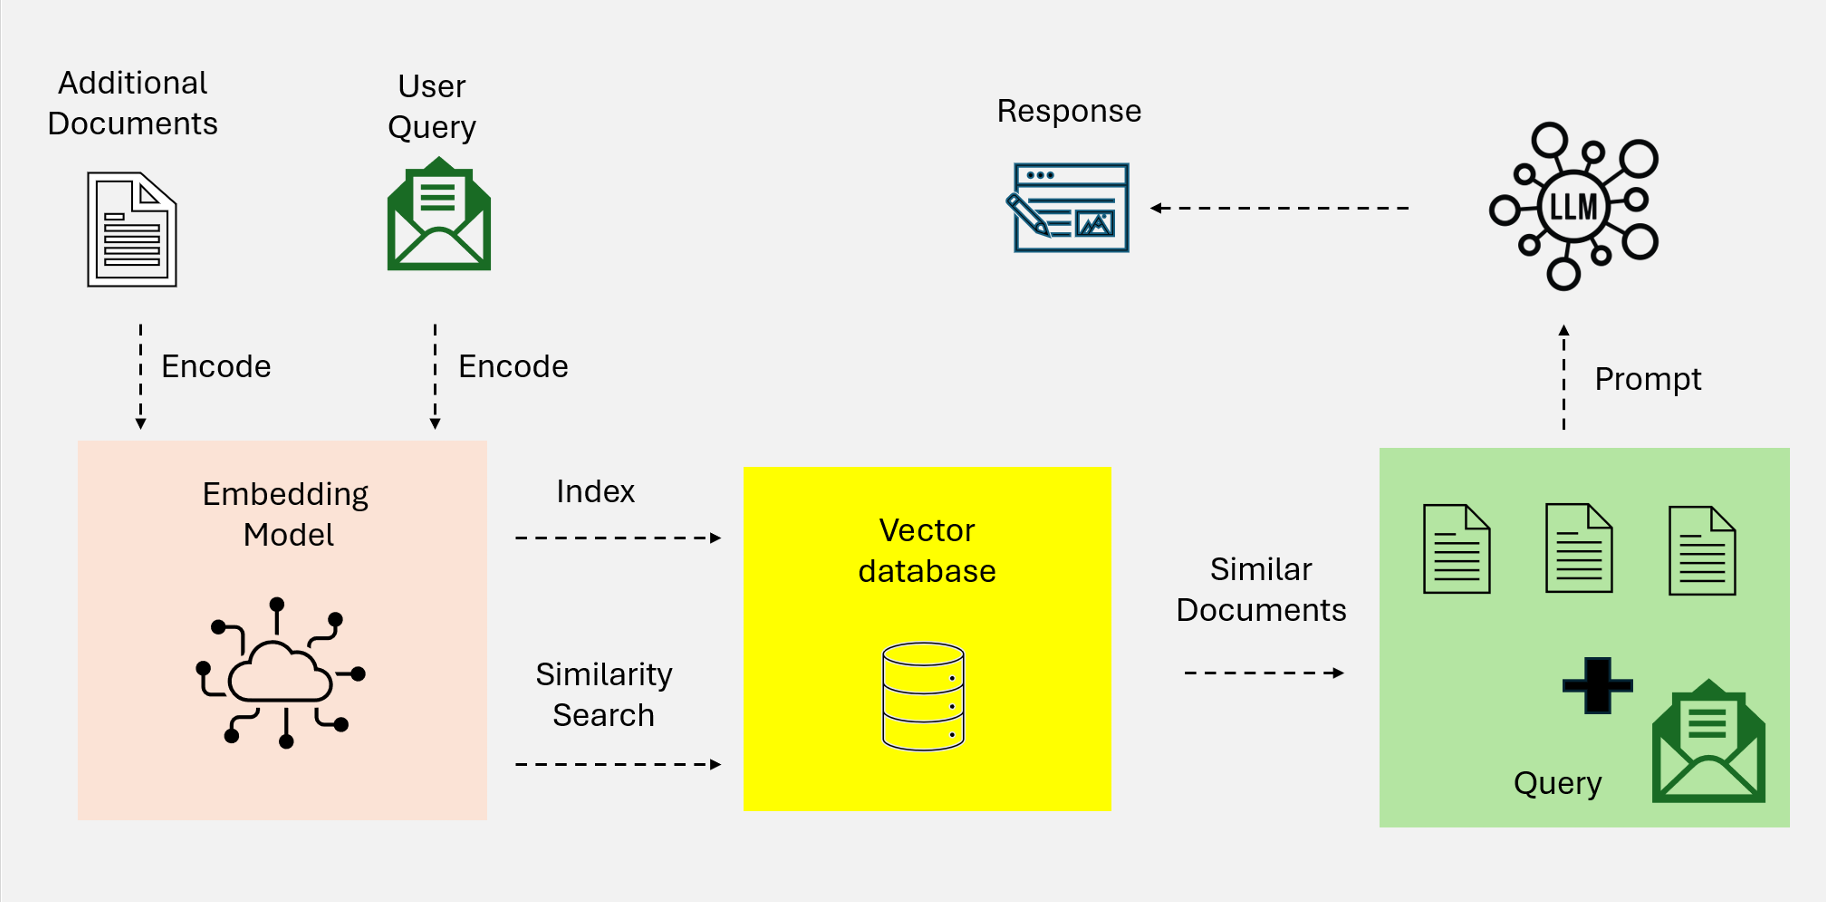
\includegraphics[width=0.85\linewidth]{images/fig_3.png}
    \vfill
    \caption{
        \textbf{Naïve RAG Architecture.}
        This diagram depicts the foundational retrieve-read workflow of Naïve RAG systems. Keyword-based retrieval methods, such as TF-IDF and BM25, are used to extract relevant documents from static datasets. The retrieved content is directly passed to the language model, which integrates this information to generate contextually enhanced responses. While effective for basic information augmentation, this architecture lacks dynamic adaptation and advanced reasoning capabilities found in more modern RAG paradigms.
    }


    \label{fig:naive_rag_architecture}
\end{figure}

Naïve RAG is characterized by its simplicity and ease of implementation, making it well-suited for tasks involving fact-based queries with minimal contextual complexity. However, it suffers from several inherent limitations:

\begin{itemize}
    \item \textbf{Lack of Contextual Awareness:} Retrieved documents often fail to capture the semantic nuances of the query due to reliance on lexical matching rather than semantic understanding.
    \item \textbf{Fragmented Outputs:} The absence of advanced preprocessing or contextual integration frequently results in disjointed or overly generic responses.
    \item \textbf{Scalability Issues:} Keyword-based retrieval techniques, such as TF-IDF and BM25, struggle with large datasets and often fail to surface the most relevant information.
\end{itemize}

Despite these limitations, Naïve RAG systems provided a critical proof-of-concept for integrating retrieval with generation, laying the groundwork for the development of more advanced and context-aware paradigms.


\subsection{Advanced RAG }

Advanced RAG \cite{gao2024retrievalaugmented}systems extend the foundational architecture of Naïve RAG by addressing its limitations through the integration of semantic retrieval and iterative reasoning capabilities \cite{lewis2020retrieval}. As illustrated in Figure~\ref{fig:advanced_rag_pipeline}, these systems adopt dense retrieval models—most notably Dense Passage Retrieval (DPR)—and neural ranking algorithms to enhance retrieval accuracy and semantic relevance \cite{karpukhin2020dense}. By embedding both queries and documents into shared high-dimensional vector spaces, Advanced RAG architectures move beyond lexical matching to enable context-aware document selection. This semantic matching substantially improves response coherence and informativeness, particularly in knowledge-intensive and multi-hop tasks.

\begin{figure}[h!]
    \centering
    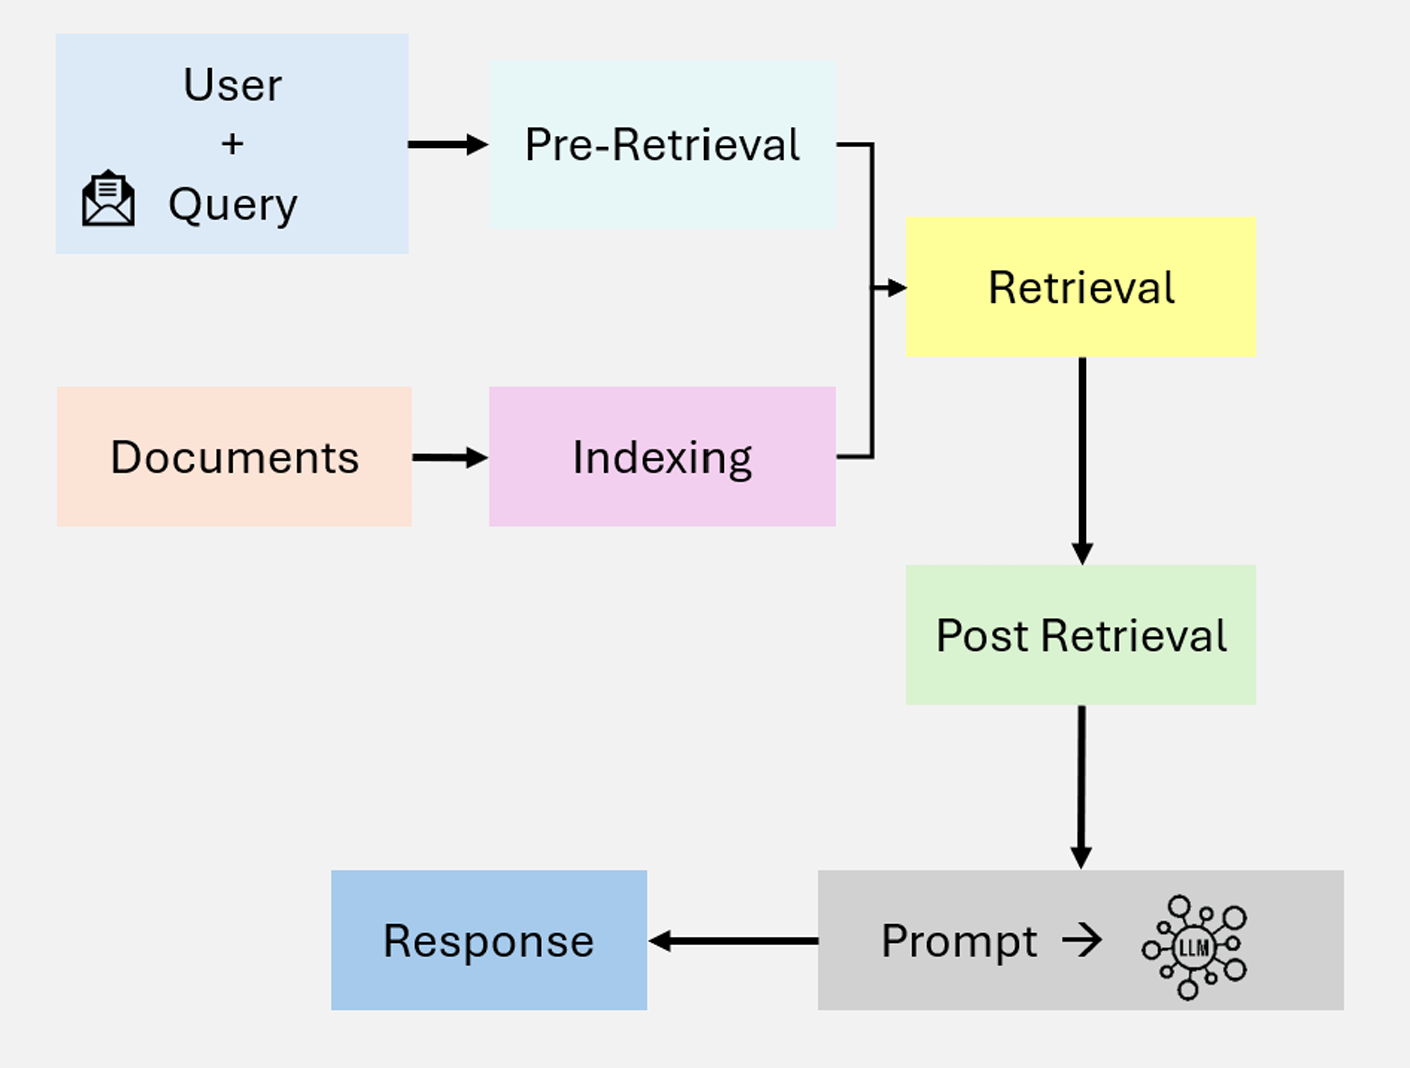
\includegraphics[width=0.9\linewidth]{images/fig_4.png}
    \caption{
        \textbf{Advanced RAG Architecture.}
        The figure showcases the enhanced workflow of Advanced RAG systems, which leverage dense retrieval models (e.g., Dense Passage Retrieval) and neural ranking to achieve semantic, context-aware document selection. Unlike Naïve RAG, this architecture supports iterative reasoning, multi-hop retrieval, and dynamic integration of retrieved knowledge, resulting in more accurate, coherent, and informative responses for complex information extraction tasks.
    }
    \label{fig:advanced_rag_pipeline}
\end{figure}


\subsection{Modular RAG }

Modular RAG\cite{gao2024retrievalaugmented} represents a significant advancement in the evolution of retrieval-augmented generation paradigms, prioritizing architectural flexibility and domain-specific customization \cite{lewis2020retrieval,shi2023replug}. Unlike earlier monolithic designs, Modular RAG systems decompose the retrieval and generation pipeline into loosely coupled, reusable components. This modularization enables more effective adaptation across diverse tasks and domains by supporting hybrid retrieval strategies, composable reasoning chains, and seamless integration of external tools. As depicted in Figure~\ref{fig:modular_rag_architecture}, such systems offer enhanced scalability and transparency, paving the way for fine-grained control over information flow and reasoning logic.

\begin{figure}[h!]
    \centering
    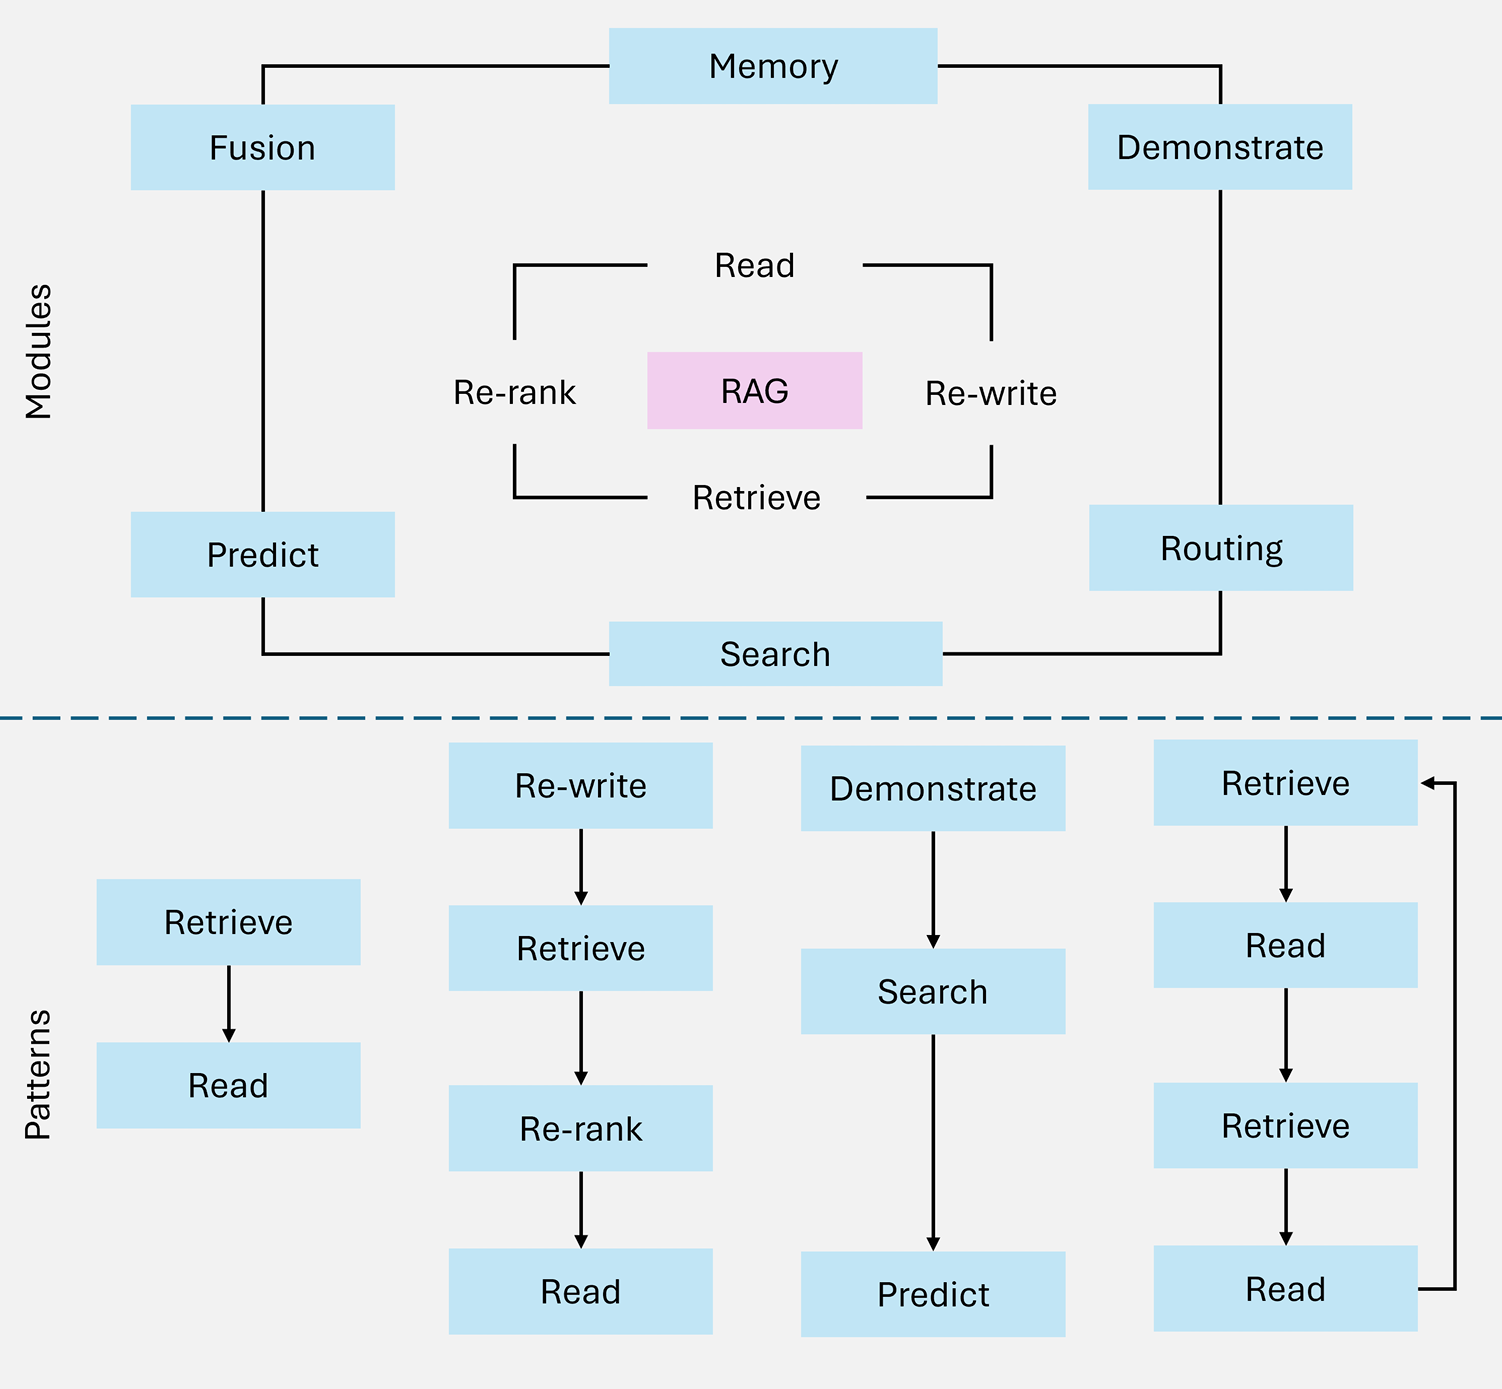
\includegraphics[width=0.92\linewidth]{images/fig_5.png}
    \caption{
        \textbf{Modular RAG Architecture.}
        This figure depicts the modular design of Modular RAG systems, where the retrieval and generation pipeline is decomposed into interoperable, reusable modules. The architecture supports hybrid retrieval (combining dense and sparse methods), composable reasoning chains, and plug-and-play integration of external tools or APIs. Such modularity enables rapid adaptation to new domains, fine-grained control over information flow, and transparent debugging and evaluation of individual components, thereby enhancing scalability, maintainability, and extensibility.
    }
    \label{fig:modular_rag_architecture}
\end{figure}

Key innovations in Modular RAG include:

\begin{itemize}
    \item \textbf{Hybrid Retrieval Strategies:} Modular RAG architectures often combine sparse retrieval methods (e.g., sparse encoders or BM25) with dense retrieval techniques such as Dense Passage Retrieval (DPR) \cite{karpukhin2020dense} to maximize accuracy across varied query types.
    
    \item \textbf{Tool Integration:} These systems incorporate external resources such as APIs, databases, or analytical tools to support real-time data processing and domain-specific computations, thereby extending the generative model's functional capacity.
    
    \item \textbf{Composable Pipelines:} A key advantage of the modular paradigm is its reconfigurability—retrievers, generators, and augmentation components can be independently replaced, enhanced, or restructured to meet the demands of specific tasks or domains.
\end{itemize}

For instance, a Modular RAG system applied to financial analytics might retrieve live stock prices via API calls, apply dense retrieval to historical market data, and generate investment recommendations through a task-specific language model. This composability and specialization render Modular RAG highly suitable for complex, multi-domain applications, offering both scalability and precision.


\subsection{Graph RAG}
Graph RAG~\cite{yao2023graphrag} extends traditional Retrieval-Augmented Generation systems by incorporating graph-based data structures, as illustrated in Figure~\ref{fig:graphrag}. These systems leverage the inherent relationships and hierarchies within graph data to support enhanced multi-hop reasoning and contextual enrichment. By integrating graph-structured retrieval, Graph RAG facilitates richer and more accurate generative outputs, particularly for tasks that require relational understanding or domain-specific knowledge traversal.

\begin{figure}[h!]
    \centering
    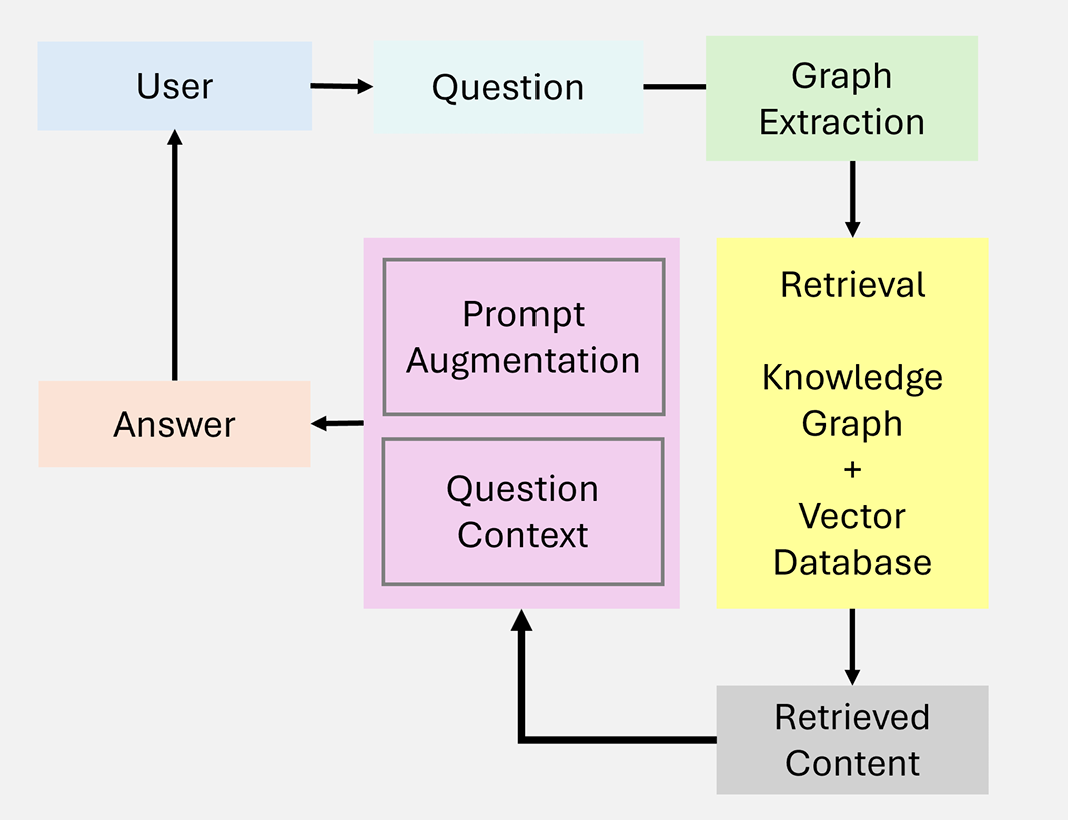
\includegraphics[width=0.92\linewidth]{images/fig_6.png}
    \caption{
        \textbf{Graph RAG Architecture.}
        This figure presents the architecture of Graph RAG systems, which integrate graph-based data structures to enable advanced multi-hop reasoning and richer contextual augmentation. By explicitly modeling relationships, entities, and hierarchies within a knowledge graph, Graph RAG systems can traverse complex information pathways, supporting more nuanced and accurate generative outputs. This approach is particularly effective for domains requiring relational understanding, such as scientific literature analysis, biomedical research, and knowledge-intensive question answering.
    }
    \label{fig:graphrag}
\end{figure}


Graph RAG is characterized by several key capabilities:
\begin{itemize}
    \item \textbf{Node Connectivity:} Enables reasoning over relationships between entities by leveraging graph link structures.
    \item \textbf{Hierarchical Knowledge Management:} Facilitates organization and inference across structured and unstructured information using graph hierarchies.
    \item \textbf{Context Enrichment:} Enhances generative responses by incorporating relational pathways derived from graph-based representations.
\end{itemize}

Despite these strengths, Graph RAG presents several limitations:
\begin{itemize}
    \item \textbf{Limited Scalability:} The reliance on explicit graph construction and traversal introduces challenges in scaling to large and evolving datasets.
    \item \textbf{Data Dependency:} The effectiveness of graph reasoning depends heavily on the availability and quality of structured graph data, making it less suitable for unstructured or noisy domains.
    \item \textbf{Integration Complexity:} Combining graph-structured reasoning with traditional unstructured text retrieval increases system complexity and requires careful design choices.
\end{itemize}

Graph RAG is particularly suitable for high-stakes domains such as healthcare diagnostics, legal research, and scientific knowledge synthesis, where structured relational reasoning is essential~\cite{yao2023graphrag}.

\subsection{Agentic RAG}

Agentic RAG represents a paradigm shift by introducing autonomous agents capable of dynamic decision-making and workflow optimization. Unlike static RAG systems, Agentic RAG incorporates iterative refinement loops and adaptive retrieval strategies to handle complex, real-time, and multi-domain queries. This approach combines the modular architecture of traditional retrieval and generation pipelines with agent-based autonomy, allowing the system to plan, select tools, and reason over multiple steps~\cite{ferrag2025can}. Agentic RAG systems are particularly well-suited for scenarios requiring tool orchestration, reflective reasoning, and continuous adaptation to evolving inputs.

Key characteristics of Agentic RAG include:
\begin{itemize}
  \item \textbf{Autonomous Decision-Making:} Agents independently evaluate and manage retrieval strategies based on query complexity.
  \item \textbf{Iterative Refinement:} Incorporates feedback loops to improve retrieval accuracy and response relevance.
  \item \textbf{Workflow Optimization:} Dynamically orchestrates tasks, enabling efficiency in real-time applications.
\end{itemize}

Despite its advancements, Agentic RAG faces several challenges:
\begin{itemize}
  \item \textbf{Coordination Complexity:} Managing interactions between agents requires sophisticated orchestration mechanisms.
  \item \textbf{Computational Overhead:} The use of multiple agents increases resource requirements for complex workflows.
  \item \textbf{Scalability Limitations:} While scalable, the dynamic nature of the system can strain computational resources for high query volumes.
\end{itemize}

Agentic RAG excels in domains such as customer support, financial analytics, and adaptive learning platforms, where dynamic adaptability and contextual precision are paramount~\cite{ferrag2025can}.

\begin{figure}[h!]
    \centering
    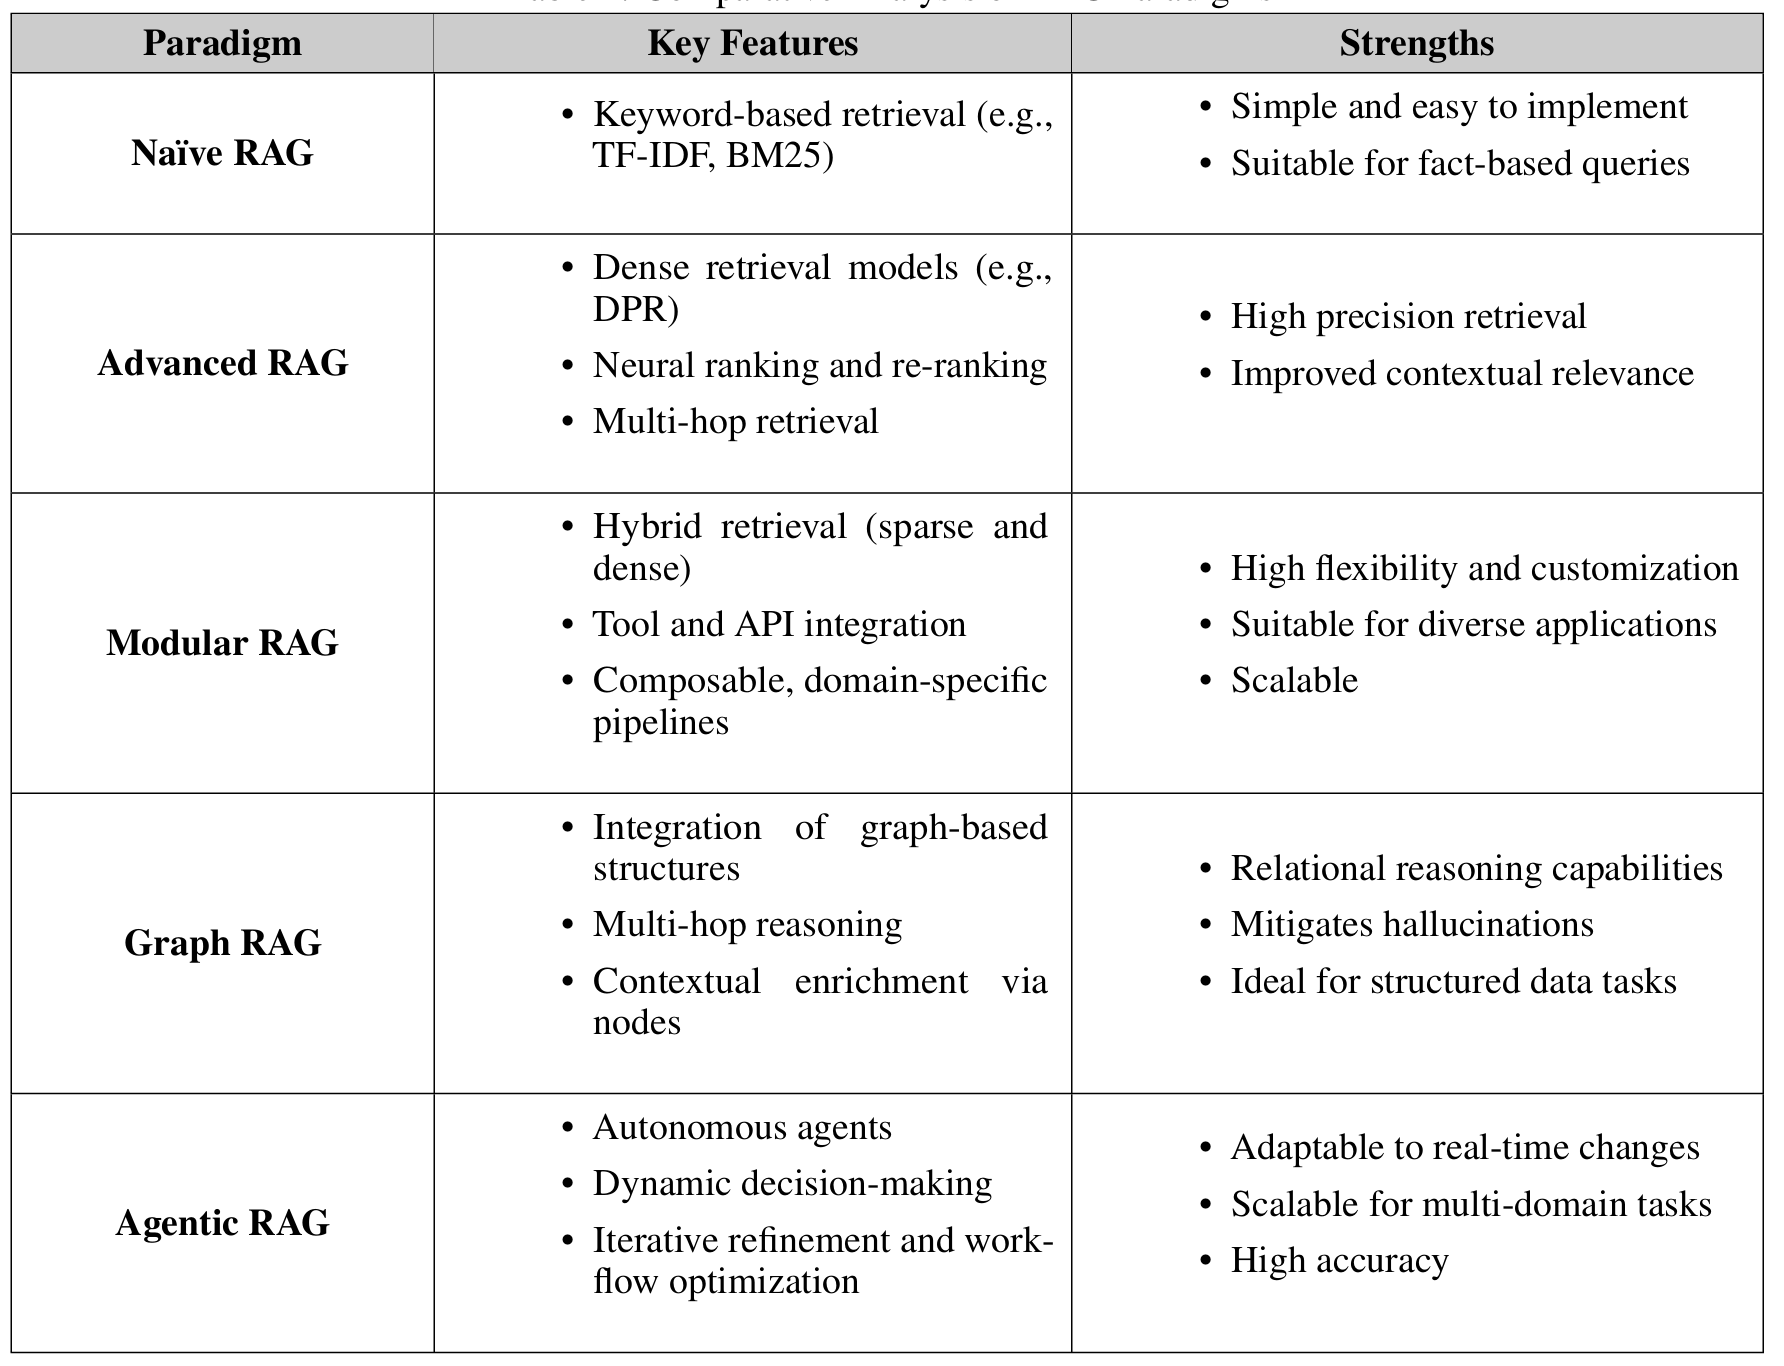
\includegraphics[width=0.9\linewidth]{images/fig_7.png}
    \caption{
        \textbf{Agentic RAG Architecture.}
        The diagram showcases the Agentic RAG system, where autonomous agents orchestrate the retrieval, augmentation, and generation modules through dynamic decision-making and workflow optimization. Unlike static RAG pipelines, the agentic controller enables iterative refinement, adaptive tool selection, and multi-step reasoning, allowing the system to respond flexibly to complex, real-time, and multi-domain queries. This architecture supports reflective reasoning, memory utilization, and continuous adaptation, making it highly effective for advanced information extraction and tool orchestration scenarios.
    }
    \label{fig:agentic_rag}
\end{figure}


\section{Agent Framework}

Agents are implemented using an open-source agent orchestration framework such as \textit{LangGraph} or \textit{AutoGen}. Each agent operates within a goal-based hierarchy, where complex tasks are decomposed into subtasks using a planning-and-reflection strategy. Agents maintain internal state and memory buffers to support multi-turn interactions, error correction, and result validation.

The classification of AI agents has evolved significantly as the field has matured, with various taxonomies proposed to categorize different agent architectures based on their capabilities, design principles, and operational characteristics. Understanding these classifications provides a framework for analyzing the strengths, limitations, and appropriate applications of different agent types~\cite{ferrag2025can}.

\subsection{Simple Reflex Agents}

Simple reflex agents represent the most basic agent architecture, operating strictly based on predefined rules and immediate perceptual data. These agents implement condition-action rules (if-then statements) that map specific environmental states to corresponding actions. As described by AWS~\cite{aws2024reflex}, simple reflex agents do not respond to situations beyond a given event-condition-action rule, making them suitable for straightforward tasks in stable, fully observable environments. Examples include thermostat controllers, basic chatbots that detect specific keywords to trigger responses, and simple automated systems for password resets. While limited in their capabilities, simple reflex agents offer advantages in terms of predictability, computational efficiency, and ease of implementation.


\subsection{Model-Based Reflex Agents}

Model-based reflex agents extend the capabilities of simple reflex agents by incorporating an internal model of the world. This model allows the agent to maintain state information that is not directly observable in the current environment, enabling more sophisticated decision-making. As noted by Russell and Norvig~\cite{russell2010aima}, model-based agents can keep track of the current state of the world and use this information to evaluate probable outcomes before selecting actions. This approach is particularly valuable in partially observable environments where the current percept alone is insufficient for optimal decision-making. Examples include navigation systems that maintain maps of their environment, recommendation systems that build user preference models, and diagnostic systems that infer internal states from observable symptoms.


\subsection{Goal-Based Agents}

Goal-based agents, also known as rule-based agents, incorporate explicit representations of desirable world states (goals) and select actions specifically to achieve these goals. Unlike reflex agents that simply react to environmental stimuli, goal-based agents engage in means-end reasoning, comparing different approaches to determine which will best achieve their objectives. According to AWS~\cite{aws2024goalagents}, these agents always choose the most efficient path and are suitable for performing complex tasks, such as natural language processing (NLP) and robotics applications. The incorporation of goals enables these agents to exhibit more flexible behavior across diverse situations, as the same goal can be achieved through different action sequences depending on environmental conditions.


\subsection{Utility-Based Agents}

Utility-based agents refine the goal-based approach by introducing a utility function that assigns values to different world states, allowing the agent to make more nuanced decisions when multiple goals conflict or when there are varying degrees of goal satisfaction. Rather than simply distinguishing between goal states and non-goal states, utility-based agents can evaluate the relative desirability of different outcomes. As AWS~\cite{aws2024utilityagents} explains, these agents compare different scenarios and their respective utility values or benefits and choose actions that provide users with the most rewards. This approach is particularly valuable for decision-making under uncertainty, where agents must balance multiple objectives or optimize across competing criteria. Examples include financial trading systems, resource allocation algorithms, and travel planning assistants that optimize across multiple preferences (e.g., cost, time, comfort).


\subsection{Learning Agents}

Learning agents represent a significant advancement in agent architecture, incorporating mechanisms to improve performance through experience. These agents modify their behavior based on feedback, gradually refining their internal models, decision rules, or utility functions to better achieve their objectives. AWS~\cite{aws2024learningagents} describes how learning agents continuously learn from previous experiences to improve results and use a problem generator to design new tasks to train themselves from collected data and past results. This capability for adaptation makes learning agents particularly valuable in complex, dynamic environments where optimal behavior cannot be fully specified in advance. Examples include recommendation systems that improve with user feedback, game-playing agents that refine strategies through practice, and conversational agents that learn from interaction histories.


\subsection{Hierarchical Agents}

Hierarchical agents organize intelligence across multiple levels of abstraction, with higher-level agents decomposing complex tasks into simpler subtasks that can be handled by lower-level agents. AWS~\cite{aws2024hierarchicalagents} describes how higher-level agents deconstruct complex tasks into smaller ones and assign them to lower-level agents, with each agent operating independently and reporting progress to its supervisor. This hierarchical organization enables the system to manage complexity through decomposition and specialization, addressing challenges that would be intractable for monolithic agent architectures. Examples include complex workflow management systems, multi-agent planning systems, and enterprise automation platforms that coordinate across multiple specialized subsystems.


\subsection{Specialized Agent Types}

Beyond these core categories, several specialized agent types have emerged to address particular application domains or capability requirements. 

\begin{itemize}
    \item \textbf{Embodied agents} integrate perception and action in physical or virtual environments, with capabilities for spatial reasoning and physical interaction.
    \item \textbf{Conversational agents} specialize in natural language understanding and generation, enabling dialogue-based interaction with users.
    \item \textbf{Collaborative agents} are designed to work effectively with humans or other agents, featuring communication, coordination, and shared task execution.
    \item \textbf{Autonomous agents} emphasize independent operation with minimal human supervision, incorporating sophisticated planning and self-management capabilities.
\end{itemize}

These specialized agents extend the versatility of AI systems, tailoring intelligence to domain-specific challenges and interaction modalities~\cite{AWS2024}.


\subsection{LLM-based Agents and Agentic AI}

The evolution of large language models (LLMs) has given rise to a new category often referred to as LLM-based agents or agentic AI. These systems leverage the reasoning capabilities of large language models while augmenting them with specialized modules for memory, planning, tool use, and environmental interaction. IBM (2024) describes how AI agents are often referred to as LLM agents and notes that while traditional LLMs produce their responses based on the data used to train them and are bounded by knowledge and reasoning limitations, agentic technology uses tool calling on the backend to obtain up-to-date information, optimize workflow, and create subtasks autonomously to achieve complex goals. This integration of LLMs with agentic capabilities represents a significant advancement in AI agent architecture, enabling more sophisticated reasoning, better contextual understanding, and more effective tool utilization~\cite{IBM2024}.


\subsection{Evolving Typology of AI Agents}

The typology of AI agents continues to evolve as new architectural approaches and combinations of capabilities emerge. Rather than constituting discrete categories, these agent types often exist along a continuum of functionalities, with many practical implementations blending elements from multiple paradigms~\cite{russell2010aima,AWS2024, IBM2024}. Understanding this typology offers a conceptual framework for analyzing the strengths, limitations, and suitable applications of various agent architectures across diverse domains, as discussed in previous sections on reflex, goal-based, utility-based, learning, hierarchical, and agentic AI agents.


\section{Tooling and Dataset}

\subsection{Retrievers}
The system employs a FAISS-based dense retriever~\cite{johnson2019billion} built over a curated corpus of RegEx patterns and relevant documentation samples. This dense retrieval method allows semantic search capabilities that outperform traditional keyword-based search, improving retrieval precision and recall in pattern extraction tasks.

\subsection{Large Language Models (LLMs)}
For generative tasks, we utilize state-of-the-art large language models including OpenAI's GPT-4-turbo~\cite{openai2023gpt4}, Mistral-7B~\cite{mistral2023}, and Google’s Gemini-Pro~\cite{google2024gemini}. These models provide advanced natural language understanding and generation capabilities, enabling dynamic interpretation and extraction of complex patterns from heterogeneous inputs.

\subsection{Agent Frameworks}
Agent orchestration is managed using LangGraph~\cite{langgraph2024}, a modular framework designed for orchestrating multi-agent workflows. Agents are implemented with Tool API wrappers~\cite{chen2023toolformer} to enable seamless integration with external tools and internal components, facilitating autonomous planning and execution.

\subsection{Corpus}
The evaluation corpus consists of a synthetic dataset comprising over 500 pattern-matching tasks derived from diverse sources such as HTML logs, CSV files, JSON documents, and unstructured free text. This dataset simulates real-world variability and complexity encountered in information extraction challenges, ensuring robust evaluation of system adaptability and accuracy.



\section{Evaluation Metrics}

To rigorously assess the performance of the proposed RAG- and Agentic AI-based framework, we adopt a comprehensive set of evaluation criteria aligned with standard practices in information extraction and natural language processing research \cite{Lewis2020RetrievalAugmentedGeneration, Karpukhin2020DensePassageRetrieval, Roberts2020BARTDenoising}.

\subsection{Accuracy}
Accuracy is measured by the exact match or semantic equivalence of extracted entities and patterns against a gold-standard annotated corpus \cite{Lewis2020RetrievalAugmentedGeneration}. This metric quantifies the correctness and precision of the extraction process.

\subsection{Flexibility}
Flexibility is assessed by the number and diversity of task formats (e.g., HTML, JSON, CSV, free text) that a single agent can successfully handle without task-specific retraining. This metric reflects the system’s generalization capability across heterogeneous input domains \cite{Karpukhin2020DensePassageRetrieval}.

\subsection{Latency}
Latency measures the average inference time per extraction task, indicating computational efficiency and feasibility for real-time applications \cite{Lewis2020RetrievalAugmentedGeneration}.

\subsection{Robustness}
Robustness evaluates the system’s ability to maintain performance under perturbed, ambiguous, or incomplete input instructions, simulating real-world noise and user error scenarios \cite{Jia2017AdversarialExamples}.

\subsection{Comparative and Ablation Studies}
Experimental comparisons are conducted against strong baselines, including traditional RegEx-only systems and LLM-only extraction methods. Ablation studies further isolate the effects of agent reasoning modules and dynamic retrieval components to quantify their contribution to overall system performance \cite{Lewis2020RetrievalAugmentedGeneration}.

Experiments compare the system against baseline regex-only and LLM-only approaches. Ablation studies analyse the contribution of agent reasoning and dynamic retrieval.











